\documentclass[10pt,twocolumn, nofootinbib]{revtex4-1}
%\documentclass[aps,pra,10pt,twocolumn,floatfix,nofootinbib]{revtex4-1}
%\documentclass[10pt,twocolumn,letterpaper]{article}

\usepackage{amsmath}
\usepackage{amsfonts}
\usepackage{graphicx}
\usepackage{enumitem}
\usepackage{hyperref}
\hypersetup{
	colorlinks=true,
	citecolor=blue,
	urlcolor=blue,
	linkcolor=blue
}
\urlstyle{same}
\DeclareMathOperator{\tr}{tr}
\frenchspacing

\begin{document}

\title{Assumptions of Physics overview:  \\
	Quantum mechanics and irreducibility}
\author{Gabriele Carcassi, Christine A. Aidala}
\affiliation{Physics Department, University of Michigan, Ann Arbor, MI 48109}

\date{\today}


\begin{abstract}
We briefly show how quantum mechanics can be rederived and better understood as a consequence of irreducibility. The Schroedinger equation (i.e. unitary evolution) is recovered as deterministic and reversible motion while the measurement process is recovered as a special case of a process with equilibria (i.e. idempotent process, projection).  This work is an overview of some of the results of Assumptions of Physics, a project that aims to identify a handful of physical principles from which the basic laws can be rigorously derived  (\url{https://assumptionsofphysics.org}).
\end{abstract}

\maketitle

\section{Introduction}

The overall argument (see \cite{AoPPhy1,AoPBook} for more details) can be summed up in the following diagram that can be used as a guide throughout this note.

\begin{figure}[h]
	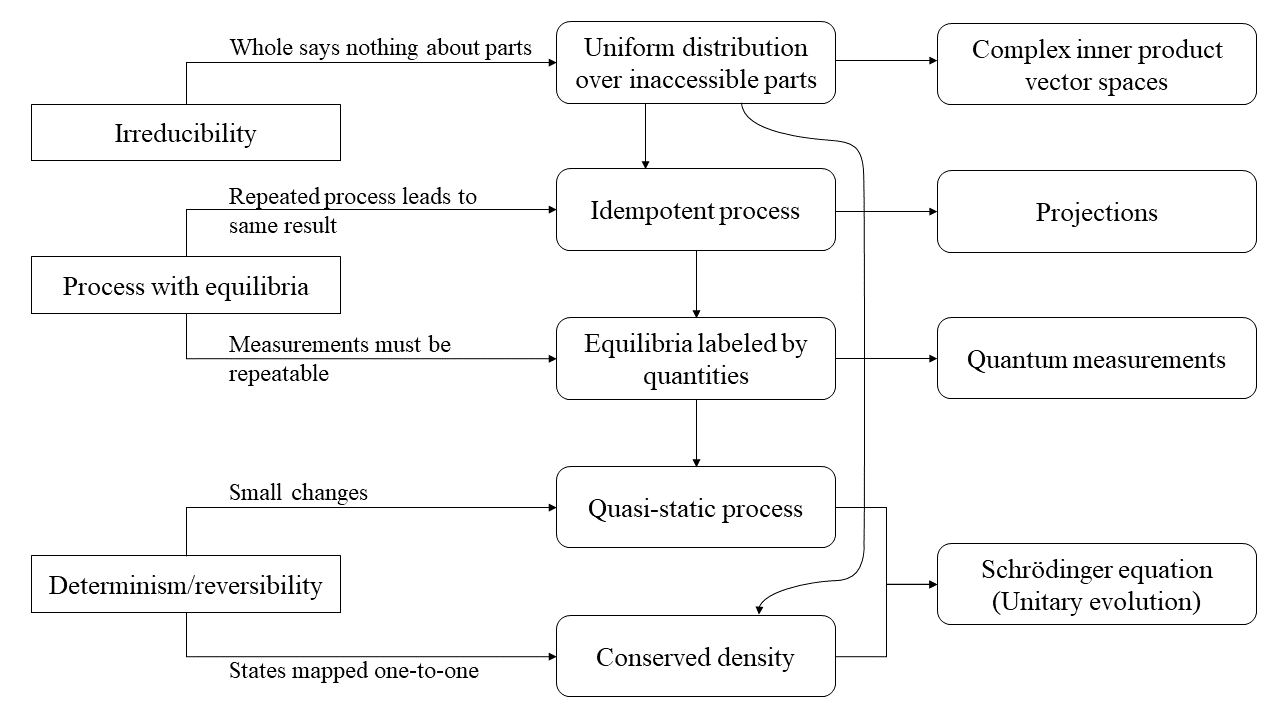
\includegraphics[width=\columnwidth]{Diagram.png}
\end{figure}

The assumptions lie on the left column. Each assumption leads to one or two key insights that progressively lead to the physical concepts in the middle column. Each of these is then mapped to its corresponding formal framework on the right. Note that ``quasi-static process'' and ``conserved density'' both independently lead to the same result of ``unitary evolution''.

\section{Irreducibility}

\textbf{Irreducibility assumption:} \emph{The state of the system is irreducible.} That is, giving the state of the whole system says nothing about the state of its parts.

Under this assumption the state of the system is automatically an ensemble over the state of the parts as preparation of the whole leaves the parts unspecified. For the same reason, the entropy of these ensembles must be the same, or some ensembles would provide more or less information about the parts. The whole task, then, is to characterize these ensembles without making specific assumptions on the parts.

Let $\mathcal{C}$ be the state space of the irreducible system. Let us call fragment a part of the irreducible system. The state of a fragment will be associated with a random variable uniformly distributed over the possible fragment states. As discussed in the context of classical mechanics(CITE), distributions over states must be invariant and symplectic manifolds are the only manifolds over which invariant distributions can be defined. As we cannot say anything about the state of the fragments, the dimensionality of this manifold must be irrelevant as long as it is even dimensional. For simplicity, we can choose a two-dimensional one. Therefore we are interested in the space of bi-dimensional uniform distributions formed by a pair of two random variables $A$ and $B$.

The values of the variables themselves are not relevant, as they are not physically accessible by assumption. However, the size of the system $\mu = \int \rho dA \wedge dB$ is relevant. Without loss of generality, we can rescale $A$ and $B$ such that the density $\rho$ is not only uniform but unitary: $\rho = 1$. This way the size of the system is directly proportional to the area covered by the random variables. In other words: the more fragments there are, the more each fragment can swap its state with another without changing the whole, the more uncertainty there is on the state of the fragment, the higher the variance of the random variables.

Since only linear transformations will preserve the uniform distribution, we look to those. These are translations, stretches and rotations. Translations do not lead to other physically distinguishable states since the exact values of $A$ and $B$ are not physically accessible. Stretching of the distribution will correspond to an increase of the size of the system, which is physically accessible. However, only the stretching of the area is of interest. So, without loss of generality, we can set $\sigma_A = \sigma_B = \sigma$ and we have $\mu \propto \sigma^2$. Rotations just change the correlations which, by themselves, are not physically accessible. However, under addition the correlations still result in differences in variance and, indirectly, the size of the system, and therefore are physically interesting. The space of transformations is therefore given by two parameters $a$ and $b$ such that:
\begin{equation}
\begin{aligned}
C &= a A + b B \\
D &= -b A + a B
\end{aligned}
\end{equation}
Equivalently, we can use the complex number $c = a + \imath b$ to characterize the transformation, which we can note as $\tau(c)$. The increase/decrease in size is given by $a^2 + b^2 = (a - \imath b) (a + \imath b) = c^* c$ and the change in correlation is given by the Pearson correlation coefficient $\rho_{A,\tau(c) A} = \cos \arg c$.

Putting it all together, we can characterize the state space $\mathcal{C}$ with a complex vector space. The linear combination represents the mixing of the different stochastic descriptions. Two vectors that only differ by a total phase are physically equivalent since a global change of correlation does not change the distribution.

We can define a scalar product $\langle \cdot | \cdot \rangle$ where the square norm induced corresponds to the size of the system (or equivalently to the strength of the random variable) and the phase difference corresponds to the correlations (the Pearson correlation coefficient). To see this, note the formal equivalence between the variance and norm rules under linear composition:
\begin{equation}
\begin{aligned}
\sigma^2_{X+Y} &= \sigma^2_{X} + \sigma^2_{Y} + 2 \, \sigma_{X} \sigma_{Y} \rho_{X,Y} \\
|\psi+\phi|^2&=|\psi|^2 + |\phi|^2 + 2 |\psi||\phi|\cos(\Delta \theta)
\end{aligned}
\end{equation}
The quadratic form, again, reflects the fact that the size of the system is proportional to the variance of a random variable. Since the size of the system is fixed, we use unitary vectors to represent actual states. The state of the system, then, is represented by a ray in a complex inner product space.

Lastly, we need to define an expectation operator that returns the average value for each physical quantity. This operator will have to be linear under linear combination of quantities:
\begin{equation}
	E[aX + bY | \psi] = aE[X | \psi] + bE[Y | \psi].
\end{equation}
 It will not be linear under linear combination of states:
 \begin{equation}
 	E[X | \psi + \phi] \neq E[X | \psi] + E[X | \phi].
 \end{equation}
Yet, it will have to be proportional to the increase in size and invariant under a total change in correlation: $E[X | \tau(c) \psi] = c^*c E[X | \psi]$. This leads us to associate to each physical quantity a linear Hermitian operator $X$ where $E[X | \psi] = \langle \psi | X | \psi \rangle$. An eigenstate $\psi_0$ of $X$ corresponds to a state where all the elements of the ensemble have exactly the same value. That is, $E[(X - \bar{x})^2 | \psi_0] = 0$.

Note that an inner product space can always be completed into a Hilbert space. This may, however, bring in objects that may not correspond to physical objects (i.e. infinite expectation for some quantities). In general, we believe it is better to regard the (possibly incomplete) inner product space as the physical state space and regard the completion as a mathematical device for calculation. For example, the Schwartz space seems more physically meaningful than the standard $L^2$ space as it gives finite expectation of all polynomials of position and momentum and, moreover, it is closed under Fourier transform.

\section{Process with equilibria}

\textbf{Process with equilibria assumption:} \emph{given an initial ensemble (i.e.~mixed state), the final ensemble is uniquely determined and remains the same if the process is applied again.}

Under this assumption, the process can be characterized by a projection operator. Let $\rho_1$ be the density matrix that characterizes a mixed state. Since the final mixed state must be uniquely determined by $\rho_1$, it will be $\mathcal{P}(\rho_1)$ for some operator $\mathcal{P}$. Similarly, if $\rho_2$ is another initial mixed state, its final operator will be $\mathcal{P}(\rho_2)$. Note that, given any observable $X$ the expectation $E[X|\rho_1] = \tr(X\rho_1)$ is the trace of $X\rho_1$. Similarly $E[X|\mathcal{P}(\rho_1)] = \tr(X \mathcal{P}(\rho_1))$.

We can always create statistical mixtures of the ensembles and we must have $E[X|a \rho_1 + b \rho_2] = a E[X|\rho_1] + b E[X|\rho_2]$ since these are classical mixtures. But since these are classical mixtures, the final state will also need to obey $E[X|a \mathcal{P}(\rho_1) + b \mathcal{P}(\rho_2)] = a E[X|\mathcal{P}(\rho_1)] + b E[X|\mathcal{P}(\rho_2)]$ for all possible $X$. Which means $\mathcal{P}(a \rho_1 + b \rho_2) = a \mathcal{P}(\rho_1) + b \mathcal{P}(\rho_2)$ Therefore the operator $\mathcal{P}$ is a linear operator. Moreover, the process applied twice must lead to the same result, which means $\mathcal{P}(\mathcal{P}(\rho)) = \mathcal{P}(\rho)$ for any $\rho$. That is, $\mathcal{P}^2 = \mathcal{P}$. Therefore $\mathcal{P}$ is a projection.

Suppose, now, that we want to measure a quantity $X$. We want the final outcome, the final ensemble, to be determined by the initial state, the initial ensemble. We also want the measurement to be consistent in the sense that, if it is repeated immediately after, it should yield the same result. Therefore the process will be a projection. We will also want that the process does not distort the quantity. That is, $E[X|\rho] = E[X|\mathcal{P}(\rho)]$. This means that the eigenstates of $X$ will correspond to equilibria of the process. Moreover, subsequent measurements must give the same value, not just the same mixture. That is, if $X_1$ is the random variable after the first instance of the process and $X_2$ is the random variable after the second instance, $P(X_2 = x| X_1 = x ) = 1$. This means that $E[(X - \bar{x})^2|\mathcal{P}(\rho)] = 0$ which means the eigenstates of $X$ are the only equilibria.

The measurement process is therefore simply a special case of a process with equilibria.

\section{Deterministic and reversible evolution}

\textbf{Deterministic and reversible evolution assumption:} \emph{given the present state of the system, all future (determinism) and past (reversibility) states are uniquely identified.}

Under this assumption, the process can be characterized by unitary evolution (i.e.~the Schrodinger equation). There are multiple different ways to see this. The first relates to the more general idea that all deterministic and reversible processes must be isomorphisms in the category of states. Since the state space is an inner product space, the isomorphism is unitary evolution.

The second, is that if there is a set of quantities $X_0$ at time $t_0$ that fully identify the state (i.e. the state is the only eigenstate of those quantities), then there must be a corresponding set of quantities $X_1$ that fully identify the state at time $t_1$. This means that the evolution maps basis to basis. Moreover, given the linearity of statistical mixtures, this will also mean that a statistical distribution over $X_0$ will have to map to the same distribution over $X_1$. Therefore the evolution must map linear combinations of that basis to the same linear combination. The evolution is a linear operator. Since the total size of the irreducible system cannot change, the operator must be unitary.

The third, is by constructing a quasi-static process from processes with equilibria, much like one does in thermodynamics.  The idea is that we have an infinitesimal time step, an initial state $\psi_t$ and a final state $\psi_{t+dt}$. We want $P(\psi_{t+dt} | \psi_t ) = 1$. This means that $|\langle \psi_{t+dt} | \psi_{t} \rangle|^2 = 1$. This can happen only if the difference between initial and final states is infinitesimal. That is, $\langle \psi_{t+dt} | \psi_{t} \rangle = 1 + \imath \epsilon dt$ where $\epsilon$ is a real number. Therefore, by convention, we can write $| \psi_{t+dt} \rangle = I + \frac{H dt}{\imath \hbar} | \psi_{t} \rangle$ where $H$ is a Hermitian operator.

Putting these perspectives together, time evolution is a unitary operator which can be written as $U=e^{\frac{H\Delta t}{\imath \hbar}}$. If we start in an eigenstate of $X$, that is $X | \psi_t \rangle = x_0 | \psi_t \rangle$ we will end in an eigenstate $\hat{X} | \psi_{t + \Delta t} \rangle = x_0 | \psi_{t + \Delta t} \rangle$ of another operator $\hat{X} = e^{\frac{H\Delta t}{\imath \hbar}} X e^{- \frac{H\Delta t}{\imath \hbar}}$.

In fact:
\begin{equation}
\begin{aligned}
e^{\frac{H\Delta t}{\imath \hbar}} X e^{- \frac{H\Delta t}{\imath \hbar}}| \psi_{t + \Delta t} \rangle
&= e^{\frac{H\Delta t}{\imath \hbar}} X e^{- \frac{H\Delta t}{\imath \hbar}} U | \psi_t \rangle \\
&= e^{\frac{H\Delta t}{\imath \hbar}} X e^{- \frac{H\Delta t}{\imath \hbar}} e^{\frac{H\Delta t}{\imath \hbar}} | \psi_t \rangle \\
&= e^{\frac{H\Delta t}{\imath \hbar}} X  | \psi_t \rangle \\
&= e^{\frac{H\Delta t}{\imath \hbar}} x_0  | \psi_t \rangle \\
&= x_0 U | \psi_t \rangle \\
&= x_0 | \psi_{t + \Delta t} \rangle
\end{aligned}
\end{equation}
This is consistent with assuming there is a quasi-static process that, at every $t$, has equilibria identified by $e^{\frac{H (t - t_0)}{\imath \hbar}} X e^{- \frac{H (t - t_0)}{\imath \hbar}}$. Note that, unlike thermodynamics, the equilibria during the evolution are not set by external constraints but by the system itself. That is, $X$ depends on the initial state of the system.

In this light, the measurement processes and the unitary processes can be seen as particular cases of the same type of processes, those with equilibria, which are defined as a black-box from initial to final state. This is consistent with the irreducibility assumption as the inability to describe the dynamics of the parts implicitly assumes that the dynamics of the parts is at equilibrium and sets a time-scale under which the further description of the system (i.e. non-equilibrium dynamics) would require describing the internal dynamics.
 
\bibliography{bibliography}

\end{document}